The purpose of this documentation is to provide future developers a
road map of the most important parts of the Galant implementation. These can
be divided into several main aspects of Galant functionality:
\begin{itemize}
\item the graph data structure (Section~\ref{sec:graph_structure})
\item algorithm execution (Section~\ref{sec:execution})
\item macro expansion and compilation (Section~\ref{sec:compilation})
\item text editing and file management (Section~\ref{sec:editing})
\item graph editing and the graph window (Section~\ref{sec:graph_window})
\end{itemize}
In each case we consider sequences of events that take place as the result of
specific user or software actions, pointing out Java classes and methods that
handle the relevant functionality.

\section{Overview}

\begin{figure}
  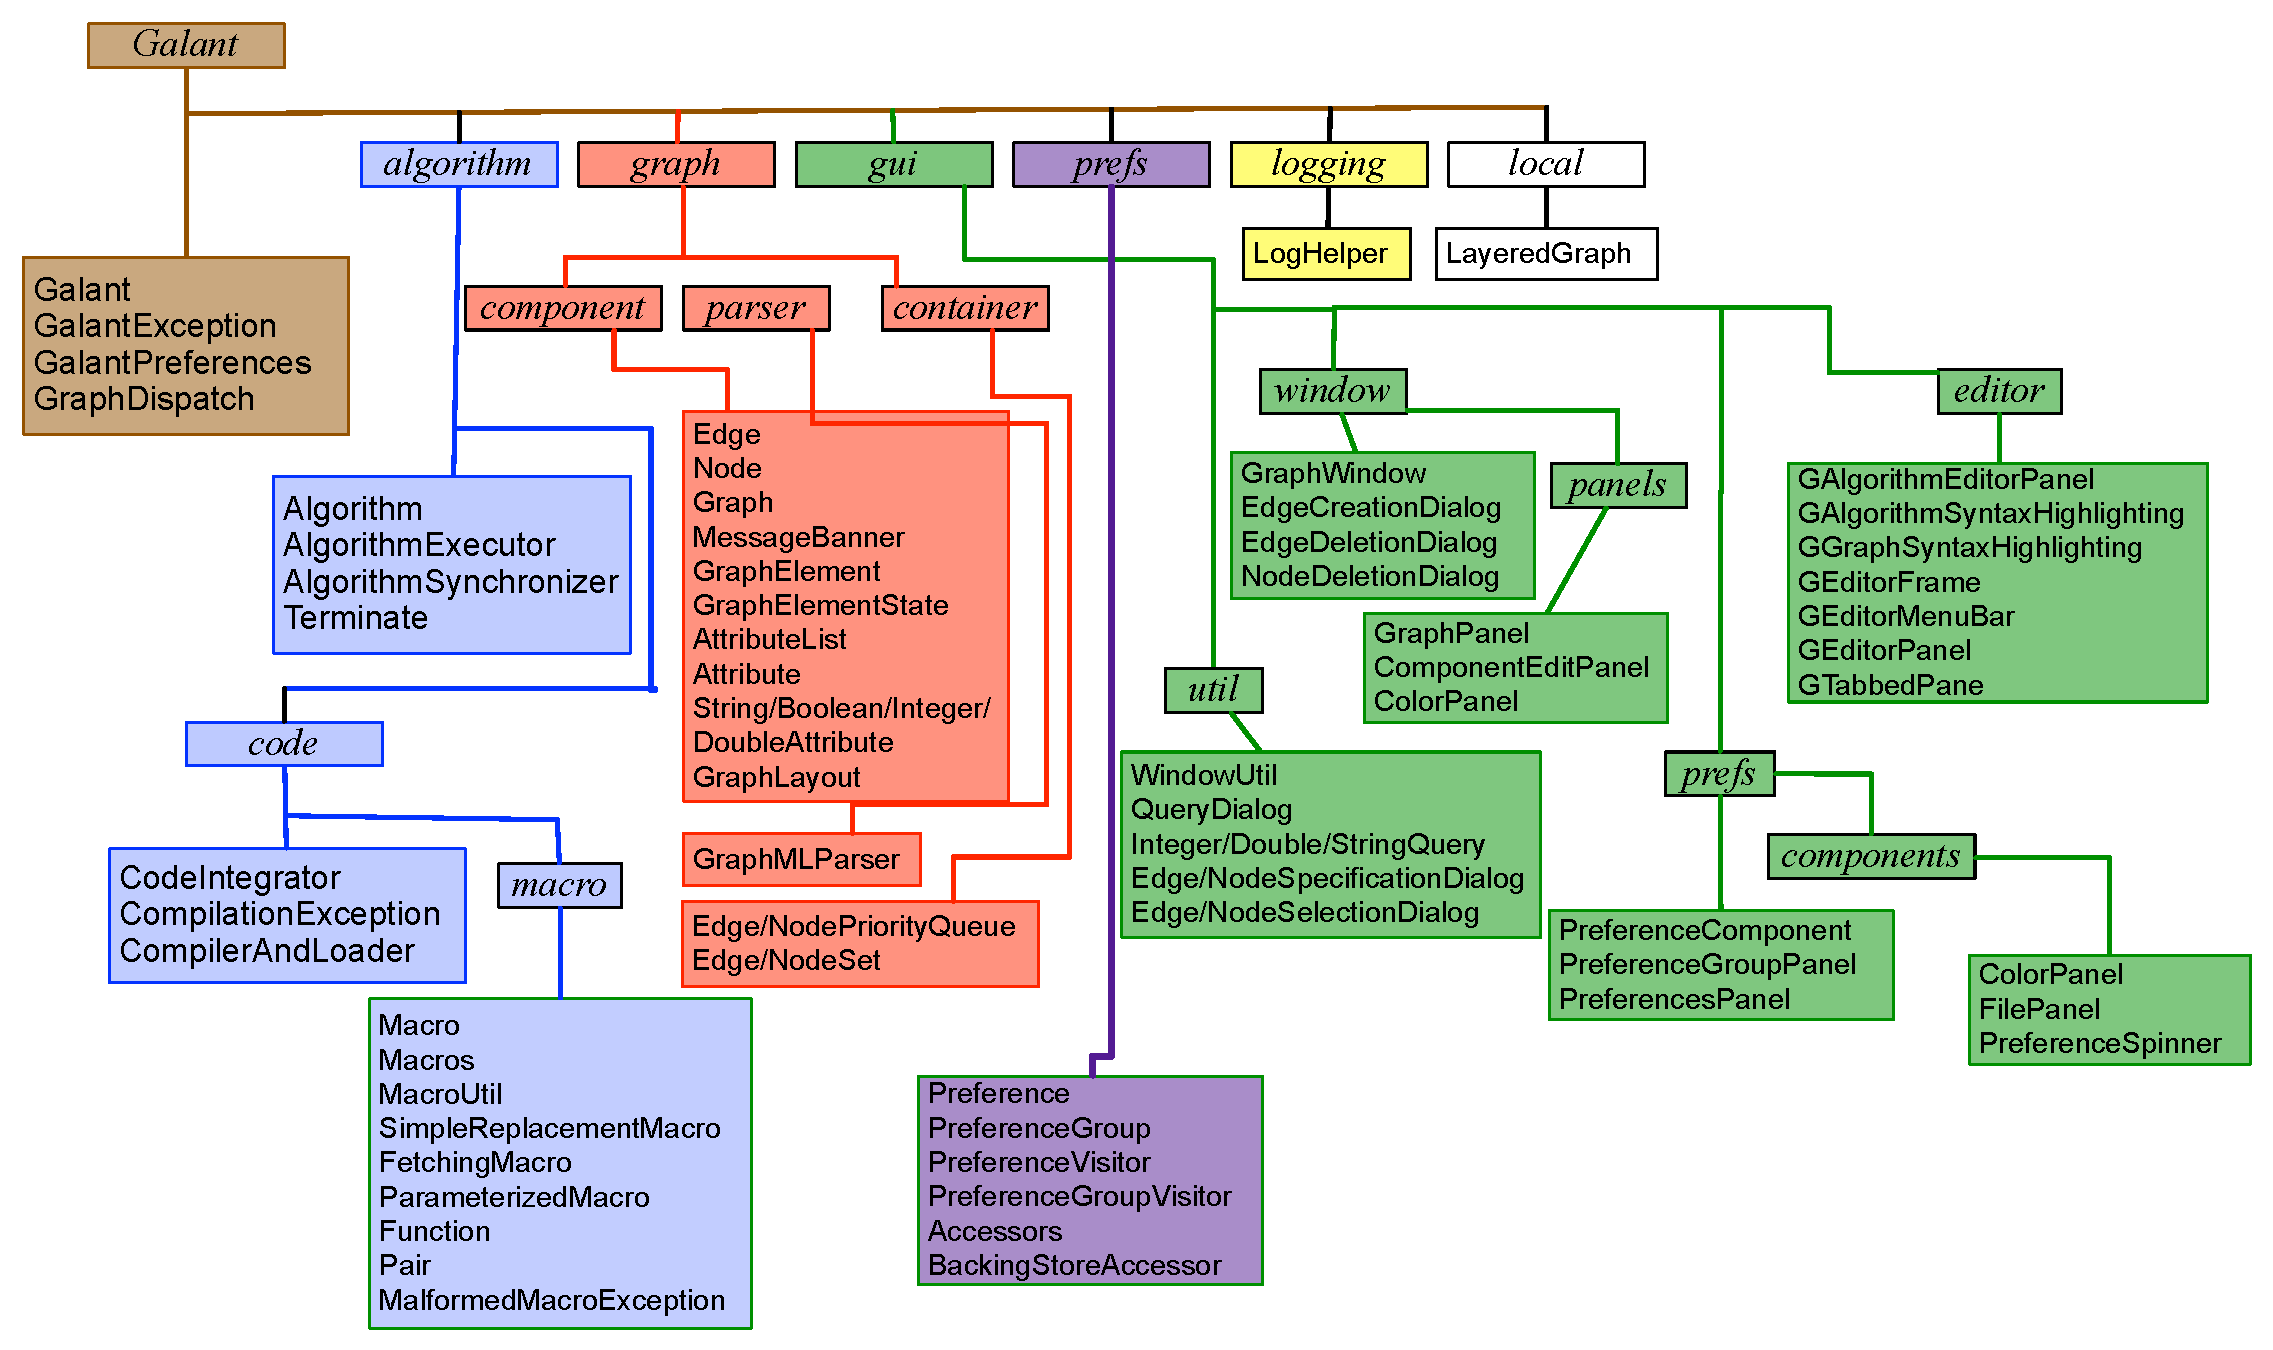
\includegraphics[width=\textwidth]{Developer/X-overview}

  \medskip
  \caption{Organization and directory structure of Galant packages.}
  \label{fig:overview}
\end{figure}

\begin{figure}

  \begin{center}
      \begin{minipage}{4in}
  \small
\begin{verbatim}
Galant.java
GalantException.java
GalantPreferences.java
GraphDispatch.java
    algorithm/
       Algorithm.java
       AlgorithmExecutor.java
       AlgorithmSynchronizer.java
       Terminate.java
       code/
          CodeIntegrator.java
          CompilationException.java
          CompilerAndLoader.java
          macro/
             FetchingMacro.java
             Function.java
             Macro.java
             MacroUtil.java
             Macros.java
             MalformedMacroException.java
             Pair.java
             ParameterizedMacro.java
             SimpleReplacementMacro.java
    graph/
       component/
          Attribute.java
          AttributeList.java
          BooleanAttribute.java
          DoubleAttribute.java
          Edge.java
          Graph.java
          GraphElement.java
          GraphElementState.java
          GraphLayout.java
          GraphState.java
          IntegerAttribute.java
          Layer.java             // not used
          LayerInformation.java  (used by Graph.java)
          LayeredGraph.java      // not used
          MessageBanner.java
          Node.java
          StringAttribute.java
       container/
          EdgePriorityQueue.java
          EdgeSet.java
          NodePriorityQueue.java
          NodeSet.java
       parser/
          GraphMLParser.java
\end{verbatim}
      \end{minipage}
  \end{center}

  \medskip
  \caption{Directory listing of Galant source code: global information,
    algorithm and graph.}
  \label{fig:directory_listing_1}
\end{figure}

\begin{figure}

  \begin{center}
      \begin{minipage}{4in}
  \small
\begin{verbatim}
    gui/
       editor/
          GAlgorithmEditorPanel.java
          GAlgorithmSyntaxHighlighting.java
          GEditorFrame.java
          GEditorMenuBar.java
          GEditorPanel.java
          GGraphEditorPanel.java
          GGraphSyntaxHighlighting.java
          GTabbedPane.java
       prefs/
          PreferenceComponent.java
          PreferenceGroupPanel.java
          PreferencesPanel.java
          components/
             ColorPanel.java
             FilePanel.java
             PreferenceSpinner.java
       util/
          DoubleQuery.java
          EdgeSelectionDialog.java
          EdgeSpecificationDialog.java
          ExceptionDialog.java
          IntegerQuery.java
          NodeSelectionDialog.java
          NodeSpecificationDialog.java
          QueryDialog.java
          StringQuery.java
          WindowUtil.java
       window/
          EdgeCreationDialog.java
          EdgeDeletionDialog.java
          GraphWindow.java
          NodeDeletionDialog.java
          panels/
             ColorPanel.java
             ComponentEditPanel.java
             GraphPanel.java
    local/
       LayeredGraph.java
    logging/
       LogHelper.java
    prefs/
       Accessors.java
       BackingStoreAccessor.java
       Preference.java
       PreferenceGroup.java
       PreferenceGroupVisitor.java
       PreferenceVisitor.java
\end{verbatim}
      \end{minipage}
  \end{center}

  \medskip
  \caption{Directory listing of Galant source code: GUI, preferences and miscellaneous.}
  \label{fig:directory_listing_}
\end{figure}

% [Last modified: 2016 12 10 at 16:52:18 GMT]


\section{Graph Structure and Attributes} \label{sec:graph_structure}

A \Code{Graph} is the container for all attributes of a graph, whether read
from a file, edited or manipulated by an algorithm.
The source code for all objects related to the structure of a graph is in
\Code{graph.component}.
Naturally, there is a list of nodes and a list of edges.
These lists are not altered in the obvious way during editing or algorithm
execution. New nodes and edges are appended to the respective lists but
deletions are virtual: a node or edge has a \Code{deleted} attribute.
New edges are also appended to the incidence lists of their endpoints:
\Code{incidentEdges} in \Code{Node}.
A graph has attributes not directly derived from its nodes or edges. These
are \Code{name} (specified by an external source), \Code{comment} (ditto),
\Code{directed} (toggled by the user but not during algorithm execution),
\Code{layered} (more details later) and \Code{banner} (message banner
displayed at the top of the graph window during algorithm execution -- see
method \Code{display()} in \Code{Algorithm}).

A node has a unique \Code{id} so that it can be referred to as an endpoint of
an edge in the GraphML representation. The map \Code{nodeById} in class
\Code{Graph} maps each integer \Code{id} to a \Code{Node} object.
The latter has an \Code{id} as one of many potential attributes.
The \Code{id}, along with a position, \Code{x} and \Code{y} attributes in
GraphML, are required for each \Code{Node}. All other attributes are
optional.
An \Code{Edge} object is required to have a \Code{source} and a
\Code{target}. If the graph is undirected, the two are interchangeable.

Both \Code{Node} and \Code{Edge} are subclasses of \Code{GraphElement} -- see
Fig.~\ref{fig:graph_uml}.
At any point in time a \Code{GraphElement} is in a particular
\Code{GraphElementState} and that state determines values of all attributes
except for the fixed ones: \Code{id}, \Code{x} and \Code{y} for \Code{Node};
\Code{source} and \Code{target} for \Code{Edge}.
A \Code{GraphElement} has a list of states to keep track of changes during
algorithm execution.
Each state is given a \emph{time stamp}\footnote{This terminology will be
  used hence to distinguish \Code{state} (as time stamp) from state as
  \Code{GraphElementState}} (the integer \Code{state}) to mark the point
during algorithm execution at which the state is effective. Currently, the
time stamp is 0 unless an algorithm is running, but could be used in a future
implementation to allow undo operations during editing.

\subsubsection*{State changes}

A \Code{GraphElement} changes state whenever any attribute changes value,
either during editing or algorithm execution. Methods of the form\\
\Code{set(String \emph{key}, \textbf{\emph{type}} \emph{value})}\\
all do the following -- see \Code{GraphElement}.
\begin{itemize}
\item create a new state \Code{newState}
\item set the attribute \emph{key} to \emph{value} in the attribute list for
  \Code{newState}
\item the setter returns \Code{true} if an attribute \emph{key} was already
  present, i.e., if an existing attribute was modified rather than a new one
  added, \Code{false} otherwise -- see \Code{AttributeList}; this Boolean
  value is available for use throughout, including by the algorithm animator
\item add the new state to the list of states in one of two ways -- see
  \Code{addState()}
  \begin{enumerate}
    \item if no state with the current time stamp exists, append the new
      state to the list of states; it becomes the most recent one, the one
      returned by \Code{latestState()}; if there is an algorithm running, the
      state change triggers the end of a step --
      \Code{pauseExecutionIfRunning()} in \Code{GraphDispatch}
    \item if there is a state with the same time stamp as the current one,
      simply replace it; this can happen during editing -- time stamp is 0,
      or if the element undergoes more than one state change during a single
      algorithm step
  \end{enumerate}
\end{itemize}
The list of states can be used to determine the attributes at any given time
(stamp) via the getters that have a \Code{state} argument. These access the
last state on the list whose time stamp precedes the given one, the
\Code{state} argument.

\begin{figure}
  \begin{center}
    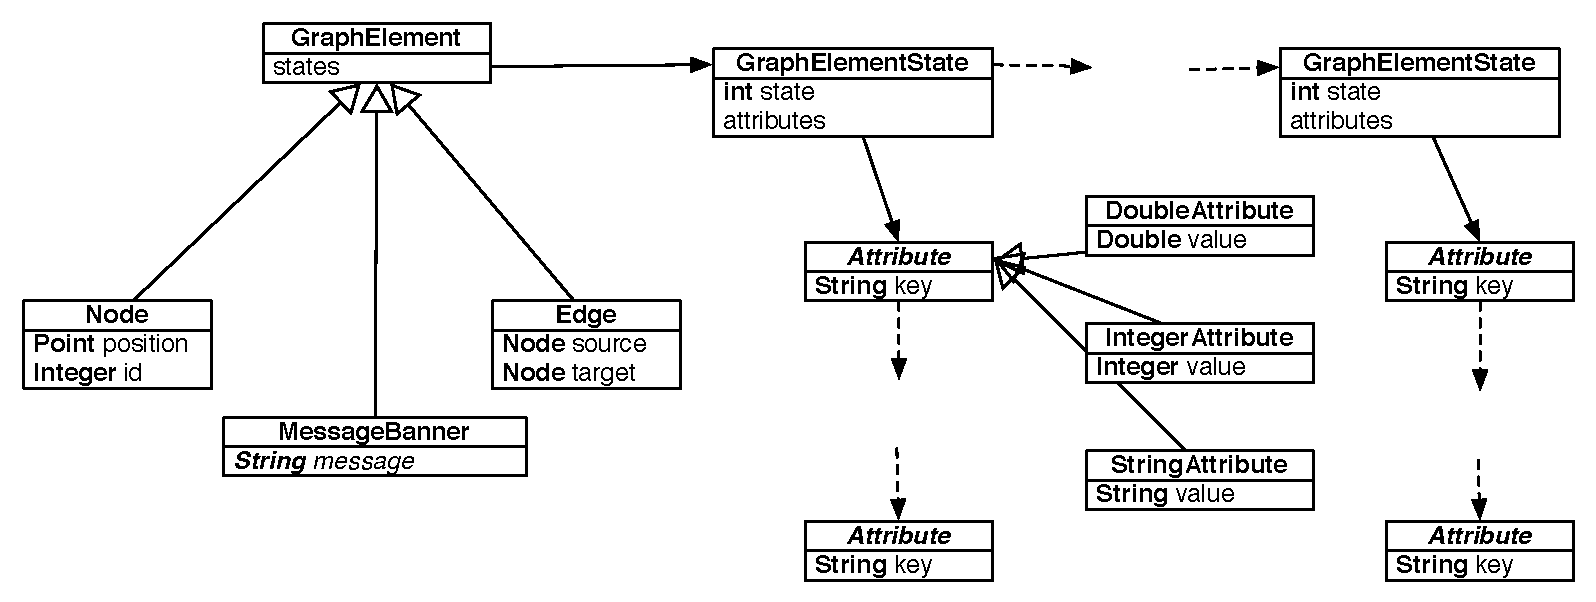
\includegraphics[width=\textwidth]{Developer/X-graph_uml}
  \end{center}
  \caption{A UML diagram showing the structure of a \Code{GraphElement}.}
  \label{fig:graph_uml}
\end{figure}

\subsubsection*{States of existence}

A node or edge may be created or deleted while editing or during algorithm
execution. To determine whether or not a \Code{GraphElement} exists at a
given point in time Galant checks its state -- the \Code{inScope()}
method. The simpler part is \Code{isDeleted()}, the predefined attribute
\Code{DELETED} = \Code{deleted}, which is set whenever the user or the
algorithm deletes the object.

To determine whether the element has already been created (this makes a
difference on in the context of algorithms that create new nodes and/or
edges) -- method \Code{isCreated(int~state)}. Here the element exists at the
given \Code{state} if there is a state on its list whose time stamp precedes
\Code{state}, i.e., if \Code{getLatestState()} returns a non-\Code{null}
value. Since an element is initialized with a single state on its list -- see
the constructor, one
whose time stamp \emph{stamp} is the time of creation, a \Code{null}
indicates that \Code{state} $<$ \emph{stamp}.

There are three contexts for \Code{Node} creation, each requiring a different
approach. All the relevant methods are in \Code{Graph}.
\begin{description}
\item[parsing] -- when reading GraphML text to create the internal
  representation of a graph, the \Code{Node} has already been initialized
  (its attributes read from the file) and it needs only to be added to the
  graph; this is accomplished by the method \Code{addNode(Node)}; the new
  node will become the \Code{rootNode} if none exists, accessible via
  \Code{getStartNode()} and sometimes used as a start node for algorithms
  that require one
\item[editing] -- in edit mode a call to
  \Code{addInitialNode(Integer,Integer)} specifies x- and y-coordinates of
  the node; a new node is created accordingly and assigned the smallest
  available id; the new node becomes the \Code{rootNode} if one is needed
\item[algorithm execution] -- the algorithm has presumably calculated a
  desired position for the node; a call to \Code{addNode(Integer,Integer)}
  has the same effect as one to \Code{addInitialNode}, but it also initiates
  a new algorithm step if appropriate
\end{description}

\subsubsection*{Types of attributes}

As already noted, \Code{Node} objects have mandatory attributes \Code{id},
\Code{x} and \Code{y} (position in the window in pixels); \Code{Edge}
objects must have \Code{source} and \Code{target}.
These must be present at all times, whether in a GraphML representation,
during editing or during algorithm execution.
The exception is the position of a \Code{Node}, which may not be specified in
a GraphML file -- if not, it is assigned randomly within window boundaries
when the file is read.

Any attribute can be specified in a GraphML file, whether or not it is
meaningful to Galant -- it might be used by an algorithm or have meaning in a
context outside Galant (so should not be discarded).
It is also possible for the animator to access and modify values of any
attributes to, for example, record the status of a node or edge during
algorithm execution. There are some predefined attributes that have an impact
on the display of a graph; a subset of these can be modified during editing
as well. All of these are defined as constants (in upper case)
at the beginning of
\Code{GraphElement}. For Boolean attributes, the absence of the attribute in
an \Code{AttributeList} is synonymous with it being \Code{false}.

Attributes that affect the display of a \Code{GraphElement} are (those marked
with * can also be edited).
\begin{description}
  \item[id] (of a node) -- displayed inside the circle representation of the
    node if it is large enough; user can set the radius as a preference
  \item[weight]* -- a floating point number that can be used for sorting or
    as a key in a priority queue (built into the \Code{compareTo()} method);
    displayed above and right of a node, in a box in the middle of an edge
  \item[label]* -- a string, displayed below and right of a node, in a box in
    the middle of an edge, to the right of the weight
  \item[color]* -- a string of the form \texttt{\#rrggbb}; each pair of
    symbols after the \texttt{\#} is a hexadecimal number indicating the
    strength of red, green or blue, respectively; predefined constants for a
    variety of colors are in \Code{Algorithm}; an edge with a defined color
    is thicker than one without; color, for a node, applies to the boundary,
    which is also thicker (thickness set by user preference) if the node has
    a color
  \item[deleted] -- if true, the element does not exist
  \item[highlighted] -- if true, the element is colored red; the color is
    determined by \Code{HIGHLIGHT\_COLOR} in
    \Code{GraphPanel}; also accessible via
    setters and getters for \Code{Selected}
  \item[marked] (node only) -- if true, the interior of the node is shaded
    using \Code{MARKED\_NODE\_COLOR} in \Code{GraphPanel}
  \item[hidden] -- if true, the element does not appear on the display
  \item[hiddenLabel] -- if true, the label of the element does not appear
  \item[hiddenWeight] -- if true, the weight of the element does not appear
\end{description}

\subsubsection*{GraphML parsing}

The \Code{GraphMLParser} (in \Code{graph.parser}) is invoked in one of three
ways listed below. The corresponding graph is then the working graph
returned by \Code{getWorkingGraph()} in \Code{GraphDispatch}.
All of the three invocations are in package
\Code{gui.editor}.
\begin{enumerate}
\item in \Code{GEditorFrame}, method \Code{updateWorkingGraph()}, called when
  the user does a \Code{Save} or \Code{Save~As} on the current panel and it
  happens to be a graph; the text in the panel has to be parsed in order for
  the changes to be reflected in the graph window -- while any edit in the
  graph window is immediately pushed to the text window, the reverse is true
  only when the text is saved
\item in the constructor for \Code{GGraphEditorPanel}, a subclass of
  \Code{GEditorPanel}, when the user opens a GraphML file; the new panel is
  created in method \Code{addEditorTab()} in \Code{GTabbedPane}
\item in \Code{GTabbedPane}, method \Code{stateChanged}, invoked when the
  user clicks on a panel containing GraphML content (either associated with a file or with an empty, unnamed graph to
  be edited by the user)
\end{enumerate}
The code for handling the panels in the text window is convoluted -- see
Section~\ref{sec:editing} -- to the extent that the three classes represented
above are opaquely intertwined. But now we will look at parsing in isolation.

\subsubsection*{Layered graphs}

The utilities in \Code{local.LayeredGraph} are used in the crossing
minimization algorithms in \Code{Research/Layered-Graphs}.
The GraphML representation of a layered graph specifies \Code{type="layered"}
and, instead of the mandatory \Code{x} and \Code{y} attributes for each node,
there are mandatory \Code{layer} and \Code{positionInLayer} attributes. In the
current implementation, layered graphs are awkwardly shoehorned into various
parts of the code. Among these are.

\begin{itemize}
\item \Code{layered} is an attribute of a graph; it might be more natural for
  a layered graph to be a subclass
\item when parsing node, a special case for layered graphs in method
  \Code{initializeAfterParsing()}; a subclass \Code{LayeredGraphNode} could
  override relevant parts of this processing
\item in \Code{GraphPanel} the method \Code{getNodeCenter()} makes a special
  case for layered graphs, calculating the position of a node so that the
  layers are distributed equally in the vertical direction and the nodes on
  each layer in the horizontal direction; a subclass could override a method
  that specifies the display position of a node appropriately
\end{itemize}

\section{Algorithm Execution} \label{sec:execution}

Algorithm execution is initiated when the user presses the \Code{Run} or
the \Code{Compile and Run} button when focused on an algorithm in the text
window. The sequence of method calls is
\begin{itemize}
\item \Code{run()} in \Code{gui.editor.GAlgorithmEditorPanel}; this
  initializes the current algorithm, the graph on which it will be run and
  the \Code{AlgorithmSynchronizer} and \Code{AlgorithmExecutor} that will be
  used to coordinate the algorithm with the GUI, respectively.

  The \Code{AlgorithmExecutor} manages the master thread, i.e., the one
  associated with the gui, and the \Code{AlgorithmSynchronizer} manages the
  slave thread, the one executing the algorithm on behalf of the user.

\item Method \Code{startAlgorithm()} in \Code{algorithm.AlgorithmExecuter}
  is called to fire up the algorithm (slave).

  At this point the gui and the algorithm behave as coroutines. The gui cedes
  control to the algorithm in
  \Code{algorithm.AlgorithmExecuter.incrementDisplayState()} and enters a
  busy-wait loop until the algorithm is done with a \emph{step} (clarified
  below) or it is terminated.

  The algorithm cedes control to the gui in
  \Code{algorithm.AlgorithmSynchronizer.pauseExecution}, where it either
  indicates that a step is finished (resulting in an exit from the busy-wait
  loop) or responds to a gui request to terminate
  the algorithm -- the gui has set \Code{terminated} -- by throwing a
  \Code{Terminate} pseudo-exception.
\end{itemize}

\begin{figure}
  \begin{center}
    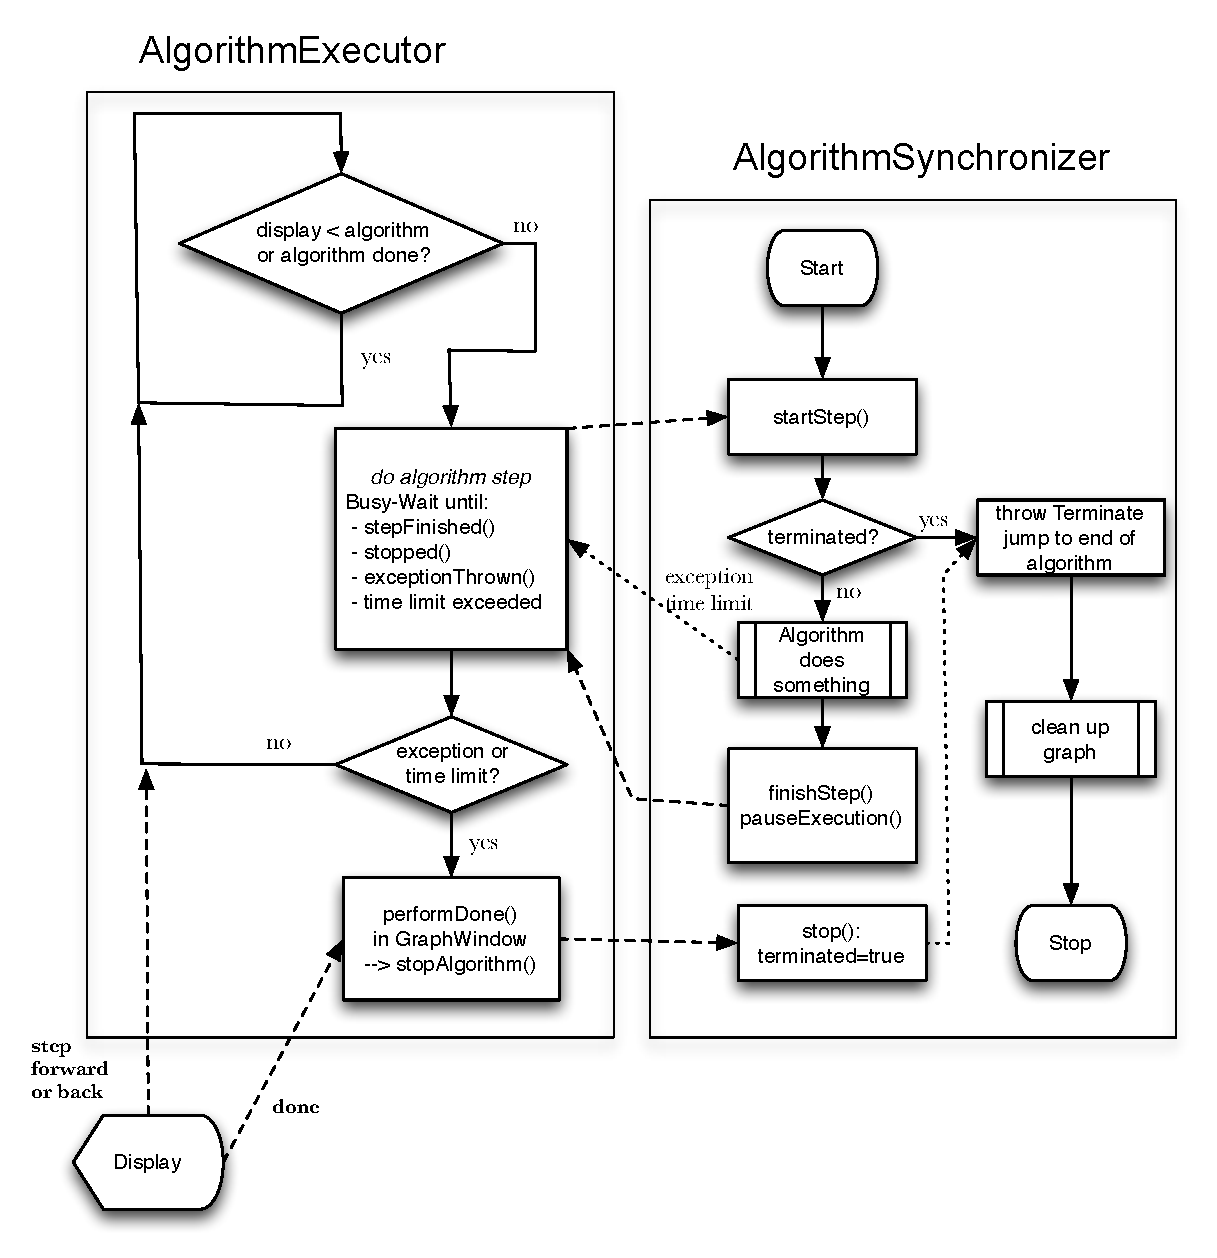
\includegraphics[width=\textwidth]{Developer/X-algorithm_execution}
  \end{center}
  \caption{Interactions between two threads during algorithm execution.}
  \label{fig:algorithm_execution}
\end{figure}

The gui controls algorithm execution, the user's view thereof, using the
buttons \Code{stepForward}, \Code{stepBackward} and \Code{done}, defined in
\Code{gui.window.GraphWindow}, or their keyboard shortcuts right arrow, left
arrow and escape, respectively.
Fig.~\ref{fig:algorithm_execution} gives a rough idea of the interaction
between the two threads (\Code{AlgorithmExecutor} and
\Code{AlgorithmSynchronizer}) that are active during algorithm execution.

\begin{itemize}
\item A step forward button press or arrow key effects a call to
  \Code{performStepForward()} in \Code{GraphWindow}, leading to an
  \Code{incrementDisplayState()}. First, there is a test,
  \Code{hasNextState()} in \Code{AlgorithmExecuter}, false only if the
  display shows the state of affairs after the algorithm has taken its last
  step.

\item \Code{incrementDisplayState()} does nothing (except increment the
  \Code{displayState} counter) if the algorithm execution is ahead of
  what the display shows (as a result of backward steps).

\item If the display state is current with respect to algorithm
  execution, the algorithm needs to execute another step -- the gui cedes
  control and enters its busy-wait loop. At this point the algorithm performs
  a step, described in more detail below.

\item A step back button press or array key effects a call to
  \Code{performStepBack()} in \Code{GraphWindow}, leading to a
  \Code{decrementDisplayState()}. The latter simply decrements the
  \Code{displayState} counter. If the display state corresponds to the
  beginning of algorithm execution -- \Code{hasPreviousState()} in
  \Code{AlgorithmExecutor} is false -- \Code{decrementDisplayState()} is not
  called.

\item The methods \Code{performStepForward()} and \Code{performStepBack()}
  also control the enabling and disabling of the corresponding buttons in the
  graph window, based on \Code{hasNextState()} and
  \Code{hasPreviousState()}. And they call \Code{updateStatusLabel()} to
  display the current algorithm and display states to the user. An algorithm
  state corresponds to a step in the algorithm.

\item A done button press or escape key leads to \Code{performDone()}, which
  in turn calls \Code{stopAlgorithm()} in the \Code{AlgorithmExecutor}.
  Here things get interesting. The \Code{AlgorithmSynchronizer} is told that
  the algorithm is to be stopped via a \Code{stop()} method call and the
  \Code{AlgorithmExecutor} cedes control to it. The algorithm is expected to
  yield control back to the executor, at which point the latter does a
  \Code{join()} to wait for the algorithm thread to finish. Algorithm and display
  states are then reinitialized to~0.

\item Complications arise with stopping the algorithm because the user may
  terminate the algorithm at any time, not just when the algorithm has run to
  completion. If it has not run to completion, the algorithm, at any
  attempt to execute the next step, checks whether it has been terminated. If so
  it throws \Code{Terminate}, an exception that is caught at the very end of
  the compiled algorithm. The effect is that of a ``long jump'' to the end of
  the algorithm.
\end{itemize}

Some complications that require extra care are:

\begin{itemize}

\item The algorithm could throw an exception. If this is a
  \Code{GalantException} the constructor informs the
  \Code{AlgorithmSynchronizer} via a call to
  \Code{reportExceptionThrown()}.
  Other exceptions may cause Galant to hang. The ultimate goal is to avoid
  these entirely. In the \Code{Algorithm} class, which defines all the
  procedural-style method calls, potential null pointer exceptions are
  caught before the underlying graph methods are called.
  The \Code{AlgorithmExecutor}, when in its busy-wait loop (or before
  entering it), checks whether
  an exception has been thrown -- \Code{exceptionThrown()} in
  \Code{AlgorithmSynchronizer} -- and terminates the algorithm if so.

\item The algorithm could get into an infinite loop. Unfortunately, under the
  current setup, an interrupt initiated by a \Code{performDone()} does not
  appear to work; so the user is not able to terminate the algorithm. The
  workaround is a time limit of \Timeout\ for the busy-wait loop, after which
  the algorithm is terminated.

\item The \Code{join()} used by the \Code{AlgorithmExecutor} to wait for the
  algorithm to finish up and the thread to terminate could cause Galant to
  hang if (i)~there was an exception; (ii)~there was an infinite loop; or
  (iii)~the animation is waiting for the user to respond to a query window.
  In cases (i) and (ii) the algorithm thread is allowed to die without being
  waited on -- see \Code{stopAlgorithm()}.

  Case~(iii), the query window, is handled by having the dispatcher maintain
  a reference to any query window that might be open --
  \Code{setActiveQuery()} and \Code{getActiveQuery()} in
  \Code{GraphDispatch}.
  The queries (all in \Code{gui.util}) are responsible for setting and
  clearing (on successful completion of the query) the reference.
  If there is an active query, as with an exception or infinite loop, the
  \Code{join()} is avoided. Also, the query window is closed.
\end{itemize}

\section{Macro Expansion and Compilation} \label{sec:compilation}

\section{Text Editing and File Management} \label{sec:editing}

\section{Graph Editing and the Graph Window} \label{sec:graph_window}

% [Last modified: 2016 12 10 at 13:54:56 GMT]
